\chapter{Results and Discussion}
\label{ch:results}

This chapter reports what the experiments found, against the objectives of Chapter~\ref{ch:intro-ref} and the protocol of Section~\ref{sec:setup}. Every table is generated from the experiment artefacts by \texttt{report/build\_assets.py}, so no result was typed by hand. Results that were unfavourable to the proposed ideas are reported with the same prominence as the favourable ones.

\section{Experimental Results}
\label{sec:experimental-results}

\subsection{Setup}
Tomato, onion, potato and ginger were studied, with 963, 511, 569 and 776 scored decision days respectively (Table~\ref{tab:dataset}). Revenue is in rupees per quintal, averaged over decision days and five farmer origins, under the default economics of Section~\ref{sec:formulation}. Brackets give 95\% day-block bootstrap intervals.

\subsection{Decision quality}

Table~\ref{tab:decision} gives mean realised revenue. In every crop the ordering is the same: nearest-mandi selling is worst; the highest price yesterday, the random walk and the boosted model trained on observed prices are close to each other; and the two models trained on realised outcomes are best. For tomato, the realised-outcome LightGBM earned Rs~2,156 per quintal against Rs~2,021 for the highest price yesterday and Rs~1,600 for the nearest mandi, with a hindsight oracle at Rs~2,570.

\begin{table}[!b]
\centering
\caption{Mean realised net revenue (Rs per quintal) with 95\% intervals; oracle shown without interval}
\label{tab:decision}
\gentable{tab_decision}
\end{table}

\begin{table}[!t]
\centering
\caption{Share of the nearest-mandi-to-oracle gap closed, and share of recommendations sent to a silent market}
\label{tab:gap}
\gentable{tab_gap}
\end{table}

\begin{figure}[!t]
\centering
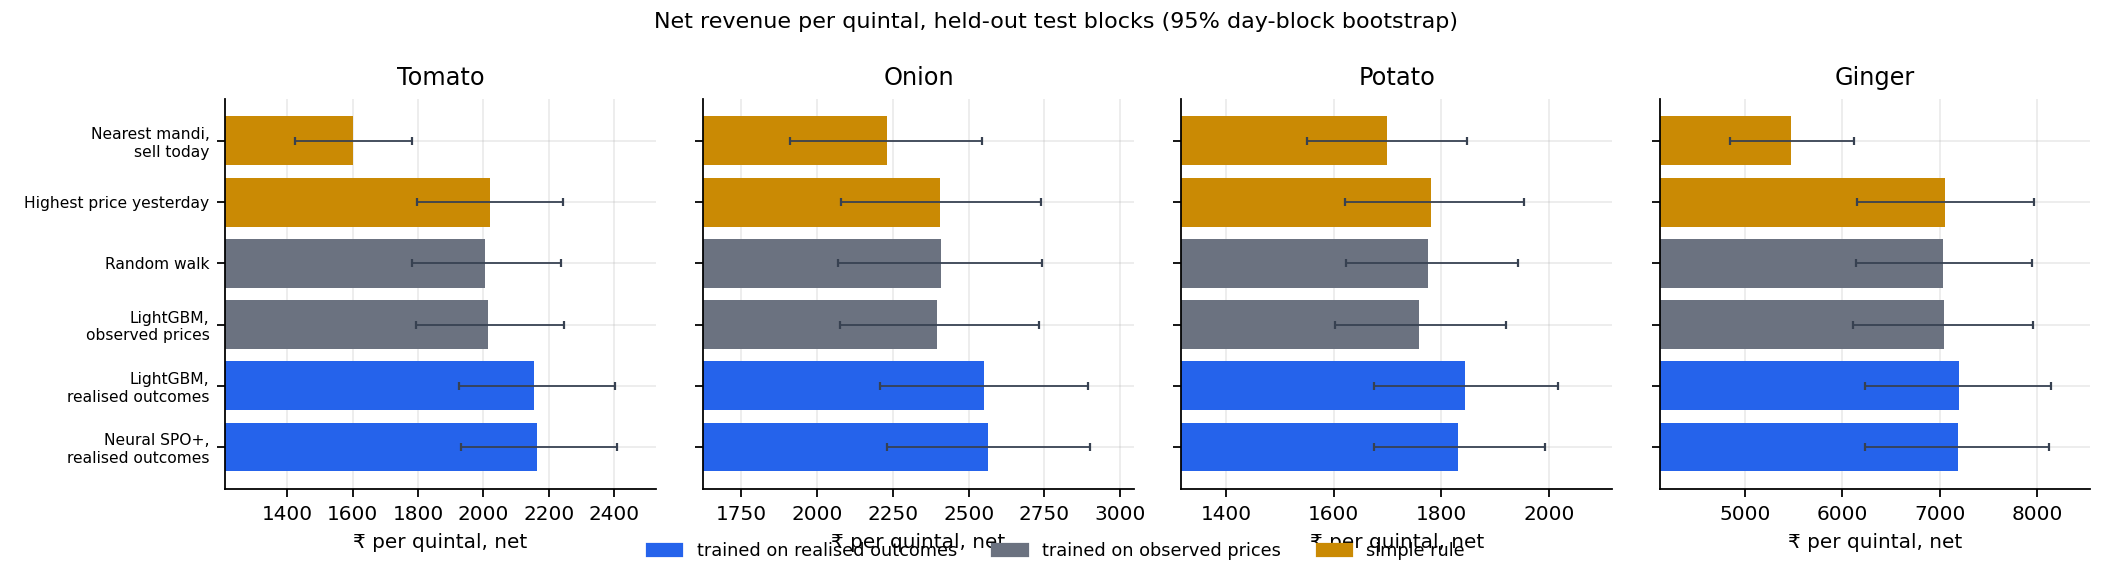
\includegraphics[width=0.85\textwidth,height=7.2cm,keepaspectratio]{figures/fig_decision_revenue.png}
\caption{Mean realised revenue by method and crop with bootstrap intervals.}
\label{fig:decision-revenue}
\end{figure}

\noindent Table~\ref{tab:gap} shows the mechanism. Models trained on observed prices sent between 12\% (ginger) and 43\% (onion) of recommendations to a market that was silent that day; the same learner trained on realised outcomes cut this by half or more (to 5--21\%). A model that never sees a silent cell cannot learn to avoid one.

\section{Performance Evaluation}
\label{sec:performance-evaluation}

\subsection{What improved decisions: the labels}
\label{sec:effects}

Table~\ref{tab:effect} isolates the two candidate causes of better decisions. Changing the \emph{labels} from observed price to realised revenue, with the same LightGBM learner, reduced regret by Rs~\LabelEffectTomato{} (tomato), \LabelEffectOnion{} (onion), \LabelEffectPotato{} (potato) and \LabelEffectGinger{} (ginger) per quintal, with Holm-adjusted $p<0.002$ in all four. The neural model showed the same effect for tomato (Rs~\LabelEffectNeural{}, interval \LabelEffectNeuralCI{}). Changing the \emph{loss} from squared error to SPO+, with labels held fixed, produced point estimates between Rs~$-66$ and $+1$ but none was reliably different from zero (Holm $p$ from 0.17 to 0.95). The honest reading is that the gain comes from learning on what the farmer actually received, and that this thesis did not find evidence for the decision-focused loss on top of it. This contradicts the expectation that SPO+ would help~\cite{elmachtoub2022} and is consistent with the finding that its benefit depends on the problem~\cite{mandi2024}.

\begin{table}[!t]
\centering
\caption{Effect of realised-outcome labels on regret (LightGBM), and of SPO+ over squared error (neural, same labels)}
\label{tab:effect}
\gentable{tab_effect}
\end{table}

\begin{figure}[!t]
\centering
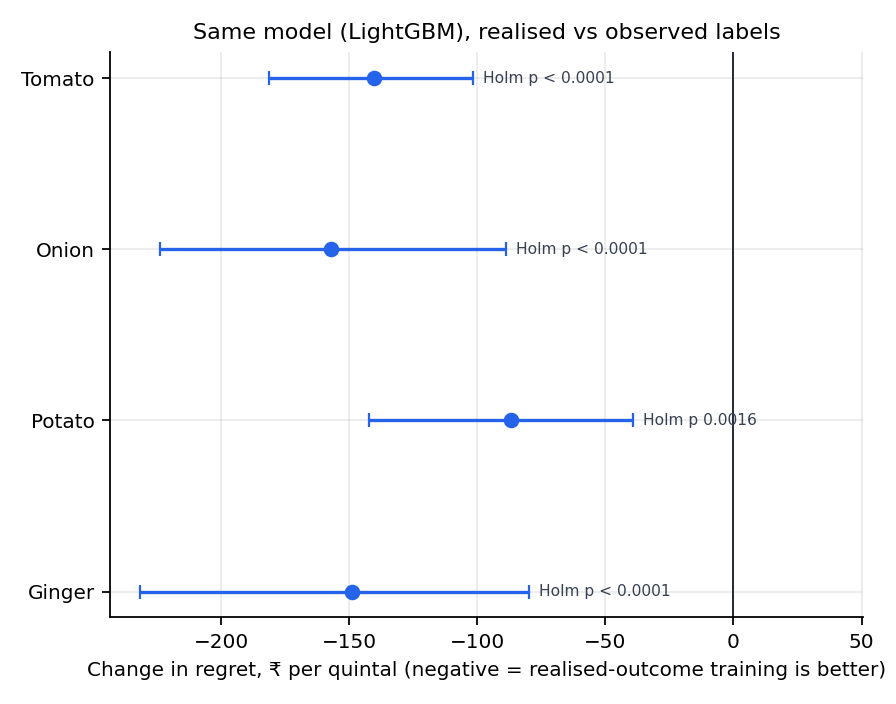
\includegraphics[width=0.85\textwidth,height=7.2cm,keepaspectratio]{figures/fig_label_effect.png}
\caption{Change in regret from realised-outcome labels, by crop, with intervals.}
\label{fig:label-effect}
\end{figure}

The model confidence set at the 10\% level retained only models trained on realised outcomes in every crop (for tomato seven specifications; for onion, potato and ginger the boosted and neural models on realised labels, with and without SPO+). No model trained on observed prices survived in any crop.

\subsection{Revenue floors}
\label{sec:floor-results}

Table~\ref{tab:floor} gives the share of days on which realised revenue fell below the stated floor. Adaptive floors were close to their targets: at a 10\% nominal level the violation rate was 9.0\% (tomato), 6.3\% (onion), 6.9\% (potato) and 10.5\% (ginger), and at 5\% and 20\% they stayed at or below the target in every crop except for marginal excesses at the 20\% level (21.3\% for tomato, 20.4\% for ginger). The static quantile was conservative, and the naive Gaussian floor, which assumes normal errors, failed badly in three crops (26--35\% violations against a 10\% target) and came closest in ginger (11.9\%). Objective 4 asked for a violation rate within two points of 10\%; this was met for tomato and ginger. For onion and potato the floors were more cautious than needed, which is the safe direction, and the objective as written was not met there.

\begin{table}[!t]
\centering
\caption{Floor violation rate (\%) on test days, served LightGBM on realised outcomes}
\label{tab:floor}
\gentable{tab_floor}
\end{table}

\begin{figure}[!t]
\centering
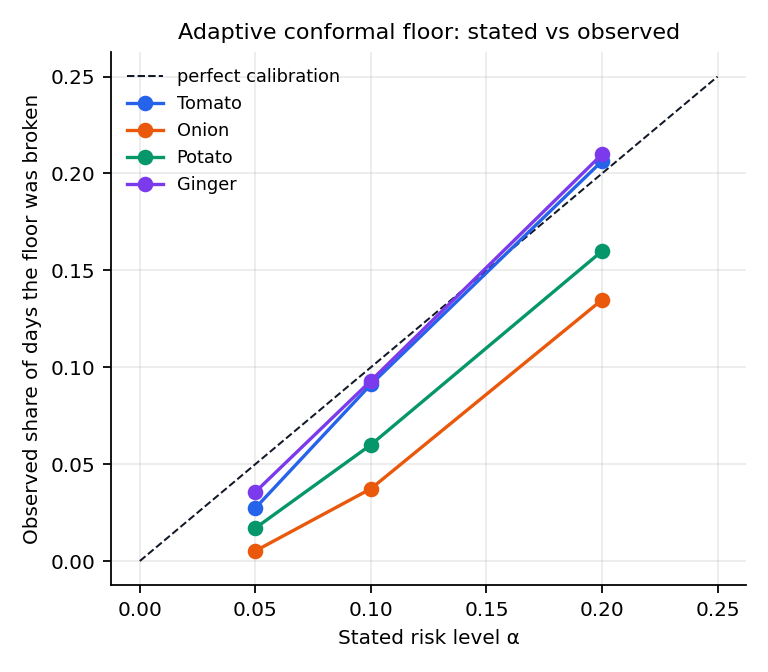
\includegraphics[width=0.85\textwidth,height=7.2cm,keepaspectratio]{figures/fig_floor_calibration.png}
\caption{Calibration of floors: observed violation against nominal level.}
\label{fig:floor-cal}
\end{figure}

\subsection{The served engines}

The engines served by the application were back-tested on the last 330 days, using only information available on each day (Table~\ref{tab:engine}). For tomato the advice earned Rs~\EngineTomatoGain{} per quintal more than the highest price yesterday, and Rs~\EngineTomatoNearest{} more than selling at the nearest mandi; ginger and onion were also significantly better than the strongest heuristic. For potato the gain over the highest price yesterday (Rs~15, interval $-38$ to $+60$) cannot be distinguished from zero, and the system labels the evidence for potato ``limited'' accordingly. Garlic is refused rather than served.

\begin{table}[!t]
\centering
\caption{Back-test of the served engines, last 330 days}
\label{tab:engine}
\gentable{tab_engine}
\end{table}

\begin{figure}[!t]
\centering
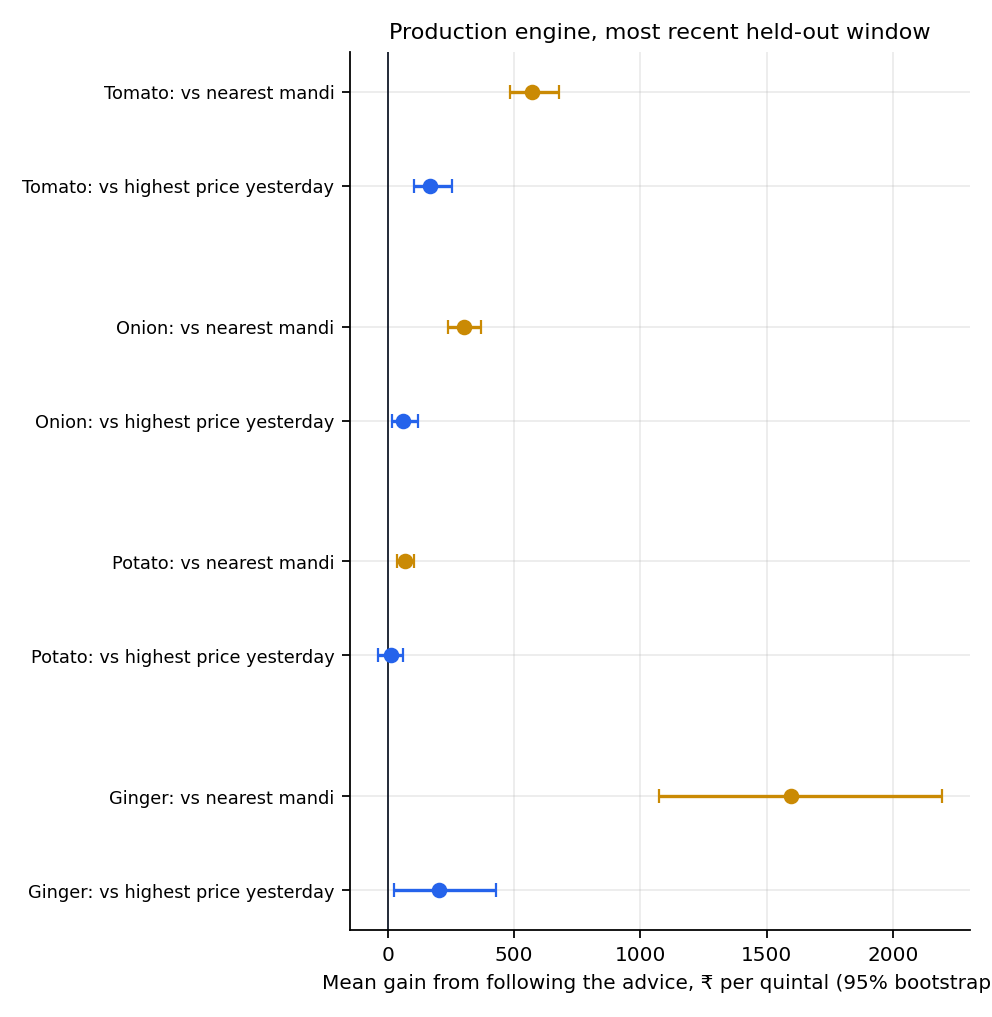
\includegraphics[width=0.85\textwidth,height=7.2cm,keepaspectratio]{figures/fig_engine_backtest.png}
\caption{Daily-backtest gain of the served advice over the two heuristic rules.}
\label{fig:engine-bt}
\end{figure}

\subsection{Price forecasts and the specialist council}

District-level forecasts of the modal price are served only where they beat no change (Table~\ref{tab:district}). The 3-, 5- and 7-day horizons showed skill of 3.0--4.0\% against no change, with direction right on 60--62\% of occasions and 90\% bands that covered 89.8\% of outcomes, at the cost of wide bands (62--75\% of the price). The 1-day horizon was not served: its skill of 0.2\% is not distinguishable from no change.

\begin{table}[!t]
\centering
\caption{District forecast report: skill against no change, direction, band coverage, and whether the horizon is served}
\label{tab:district}
\gentable{tab_district}
\end{table}

Table~\ref{tab:forecast} compares a single model, a linear stack and the specialist council on market-level forecasts. The council improved on the single model in only one of four folds at 3 and 5 days and in none at 7 days, and its average skill (+0.2 to +0.4\%) did not exceed the single model's (+0.6 to +0.8\%). The council was therefore not promoted to the served system; it is retained as an inspectable diagnostic. Table~\ref{tab:council} shows the weights: the trend agent carried most weight and the seasonal agent, alone, was worse than no change.

\begin{table}[!t]
\centering
\caption{Skill against no change: single model, linear stack (ElasticNet), equal-weight agents and weighted council. ``Folds won'' counts the folds in which the single model beat no change}
\label{tab:forecast}
\gentable{tab_forecast}
\end{table}

\begin{table}[!t]
\centering
\caption{Skill and mean weight of each specialist agent}
\label{tab:council}
\gentable{tab_council}
\end{table}

\begin{figure}[!t]
\centering
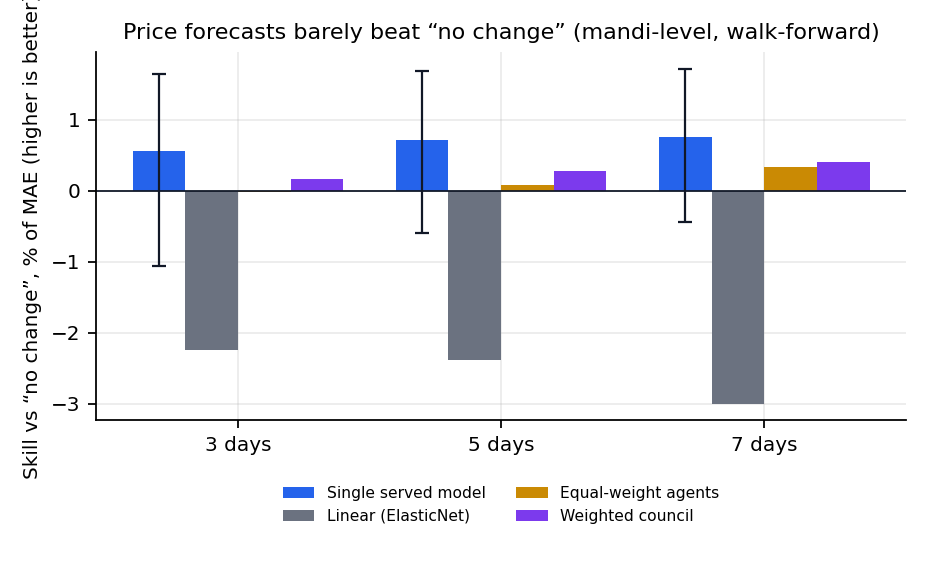
\includegraphics[width=0.85\textwidth,height=7.2cm,keepaspectratio]{figures/fig_forecast_skill.png}
\caption{Forecast skill against no change across horizons.}
\label{fig:forecast-skill}
\end{figure}

\subsection{Explaining and stress-testing the advice}
\label{sec:insight-results}

Table~\ref{tab:breakdown} is the breakdown for tomato at Kolar with 10 quintals: its parts add up to the served net revenue (a test requires it). The advice, \AdvMandi{} after \AdvDays{} day, nets Rs~\AdvNet{} per quintal against Rs~\NearNet{} at the nearest mandi: the price it expects is Rs~776 higher, and that outweighs its extra transport (Rs~94) and spoilage (Rs~60). Table~\ref{tab:whatif} stress-tests it. Raising transport to Rs~3.0 per quintal-km, over four times the tempo rate, lowers the net to Rs~1,515 but does not change the advice (\TransportFlips{} changes anywhere between Rs~0.1 and Rs~3.0). The advice does change when spoilage reaches \SpoilFlipAt\% a day, or when the farmer cannot wait: it becomes \AdvMandi{} on the same day, Rs~1,789. A farmer can therefore see that the advice is robust to the truck and fragile to the crop's shelf life.

\begin{table}[!t]
\centering
\caption{Breakdown of the advice and its alternatives, tomato at Kolar, 10 quintals (Rs per quintal)}
\label{tab:breakdown}
\gentable{tab_breakdown}
\end{table}

\begin{table}[!t]
\centering
\caption{The advice under other costs (tomato at Kolar)}
\label{tab:whatif}
\gentable{tab_whatif}
\end{table}

\subsection{Track record on days the advice had not seen}
\label{sec:track-results}

Table~\ref{tab:track} replays the advice over \TrackDays{} out-of-sample days (\TrackFrom{} to \TrackTo). Against the nearest mandi the advice won on 93\% of days for tomato, 82\% for onion, 63\% for potato and 90\% for ginger. Against the highest price yesterday most days are ties, because the advice often picks the same action; where it differs it wins more often than it loses for tomato (24\% against 8\%) and onion (34\% against 27\%), as often as it loses for ginger (23\% each), and wins 52\% against 36\% for potato, by small amounts. The floor, set to hold on nine days in ten, held on \FloorTomato\% (tomato), \FloorOnion\% (onion), \FloorPotato\% (potato) and \FloorGinger\% (ginger) of the replayed days. This is below target for tomato, onion and ginger. Table~\ref{tab:floorcmp} puts the three views of the same question side by side: the served rule's back-test over 330 days (9.6 to 12.3\% violations), a static multiplier evaluated out of sample (7.8 to 17.7\%) and this replay, which fits one multiplier on a half-window and is therefore the strictest (8 to 16\%). The floors are close to their level but not exactly at it, and a farmer is told so on the screen (Figure~\ref{fig:ui-insight}c).

\begin{table}[!t]
\centering
\caption{Replay of the advice on out-of-sample days}
\label{tab:track}
\gentable{tab_track}
\end{table}

\begin{figure}[!t]
\centering
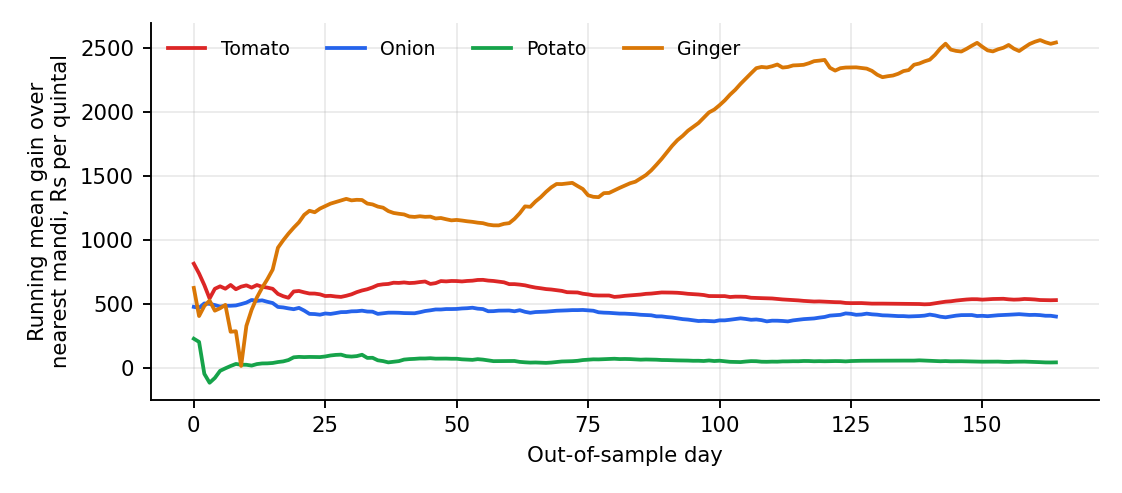
\includegraphics[width=0.82\textwidth]{figures/fig_track.png}
\caption{Running mean gain of the advice over the nearest mandi, by crop, on out-of-sample days.}
\label{fig:track}
\end{figure}

\begin{table}[!t]
\centering
\caption{Floor violation (target 10\%) under three evaluations}
\label{tab:floorcmp}
\gentable{tab_floorcmp}
\end{table}

\subsection{Silence tax}

Over \SilenceMandis{} tomato mandis, a trip loses Rs~\SilenceMean{} per quintal on average to unexpected silence. The costliest is \SilenceTopName{}, at Rs~\SilenceTopLoss{} per quintal (\SilenceTopPct\% of its price): it reported on 44\% of days and is silent on Sundays, on top of which it is unpredictably silent on other days (Table~\ref{tab:silence}). Chikkaballapur reported on none of the Thursdays in the last year (\ThursdayChik\% silent), so it is treated as closed that day, and a farmer is warned not to take a Thursday load there. A tax of Rs~0 for cheap mandis such as Kolar does not mean they are reliable; it means their usual price is below the fallback, so silence costs no money on price. Figure~\ref{fig:silence} shows every mandi by weekday. A day with no price may be a closed mandi or a missed upload, which the portal does not distinguish.

\begin{table}[!t]
\centering
\caption{Silence tax per mandi, tomato, last 365 days}
\label{tab:silence}
\gentable{tab_silence}
\end{table}

\begin{figure}[!t]
\centering
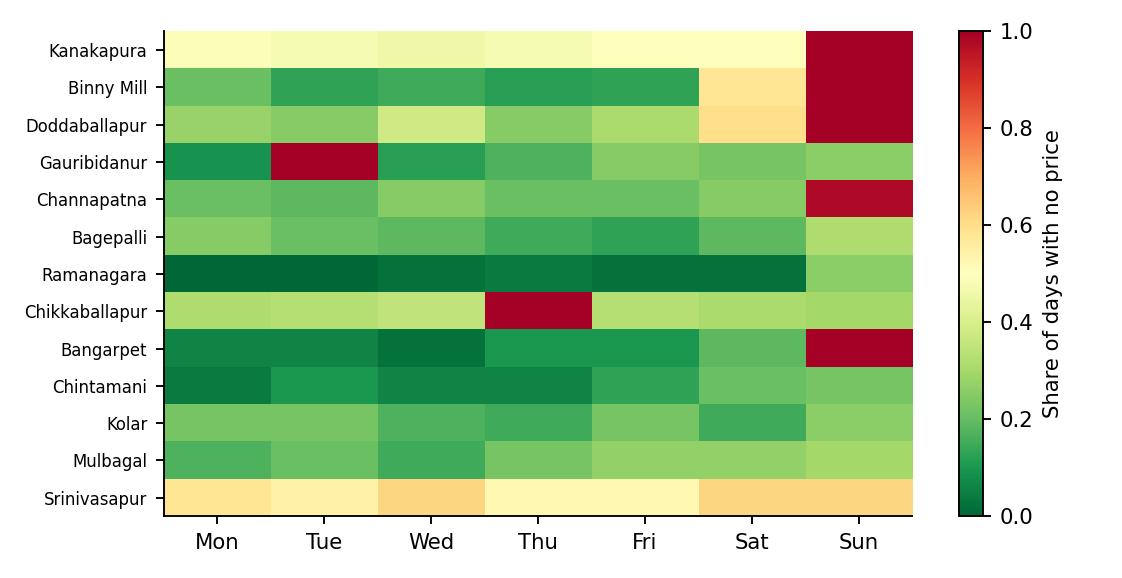
\includegraphics[width=0.85\textwidth]{figures/fig_silence.png}
\caption{Share of days on which each tomato mandi reported no price, by weekday. Red columns are days a mandi is effectively closed.}
\label{fig:silence}
\end{figure}

\subsection{What happens when many farmers follow the advice}

Table~\ref{tab:crowd} and Figure~\ref{fig:crowd} show the effect for 10 quintals per farmer, tomato, Kolar farmers. A single farmer nets Rs~\CrowdAlone{} per quintal. If 200 farmers (2,000 quintals) all follow the advice, the best yard, which usually receives about \CrowdYard{} quintals a day, sees its price fall by \CrowdDrop\% and each farmer nets Rs~\CrowdBest{}, which is no better than everyone going to the nearest mandi (Rs~\CrowdNearest{}). A coordinated split, telling farmers different actions with the stated probabilities, nets Rs~\CrowdCoord{}: Rs~\CrowdGain{} per quintal more, Rs~\CrowdTotal{} for the group. As the crowd grows to 2,000 farmers every policy deteriorates and coordination matters more. Table~\ref{tab:crowdb} shows how much of this depends on the assumed price flexibility $b$: with $b=0$ the crowd costs nothing and all policies are equal, and the conclusion strengthens as $b$ rises. This is a scenario, not a measurement: the flexibility is an association in past data and the real response to a crowd of advised farmers has not been observed.

\begin{table}[!t]
\centering
\caption{Net revenue per quintal (Rs) under four policies as the crowd grows, tomato, Kolar farmers, 10 quintals each}
\label{tab:crowd}
\gentable{tab_crowd}
\end{table}

\begin{figure}[!t]
\centering
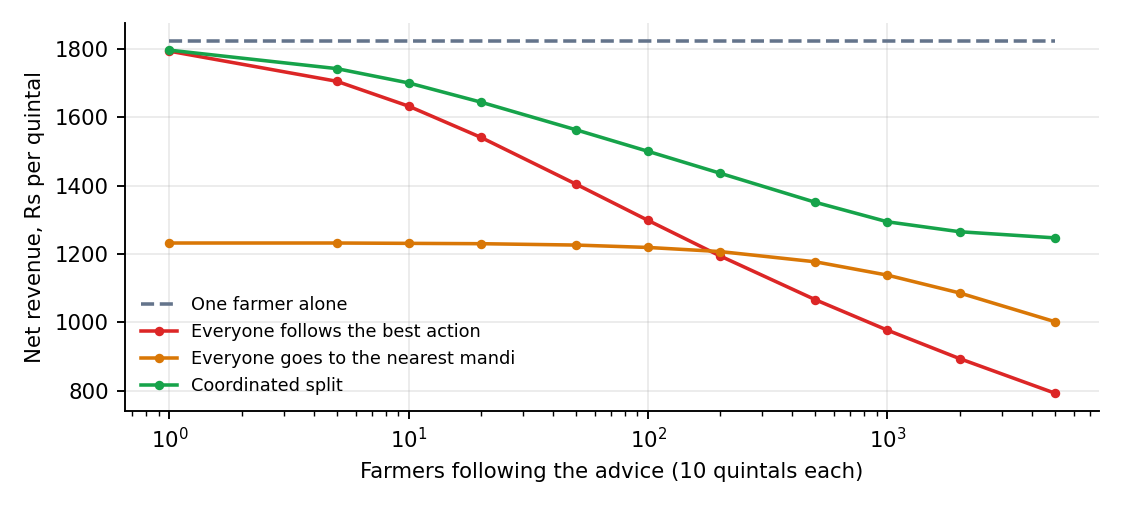
\includegraphics[width=0.82\textwidth]{figures/fig_crowd.png}
\caption{Net revenue per quintal against the number of farmers following the advice.}
\label{fig:crowd}
\end{figure}

\begin{table}[!t]
\centering
\caption{Sensitivity to the price flexibility $b$, 200 farmers}
\label{tab:crowdb}
\gentable{tab_crowdb}
\end{table}

\section{Validation}
\label{sec:validation}

\subsection{Leakage audit of decompose-then-forecast models}
\label{sec:leakage}

Table~\ref{tab:leak} compares the published protocol, in which the series is decomposed once over its whole length, with a causal protocol that decomposes only data available at each forecast origin, for tomato. The published protocol reports skill against the random walk of +27\% to +62\%. Under the causal protocol the same models score between $-15\%$ and $-1\%$, no better than the raw series ($-14\%$ to $-1.5\%$). The difference, 30 to 71 points with intervals that exclude zero, is look-ahead leakage: STL and VMD are two-sided smoothers, so the component at day $t$ already contains the prices that follow it. A zero-shot foundation model was also worse than no change (skill \ChronosOne{}\% at one day and \ChronosSeven{}\% at seven days), so no model in this comparison beat the random walk on the daily tomato series. We did not audit the specific published studies; the claim is about the protocol they describe.

\begin{table}[!t]
\centering
\caption{Forecast skill against the random walk (\%), tomato. Published: series decomposed once over its whole length; causal: decomposed only on data available at each origin; raw: no decomposition. Gap: published minus causal, in percentage points}
\label{tab:leak}
\gentable{tab_leak}
\end{table}

\begin{figure}[!t]
\centering
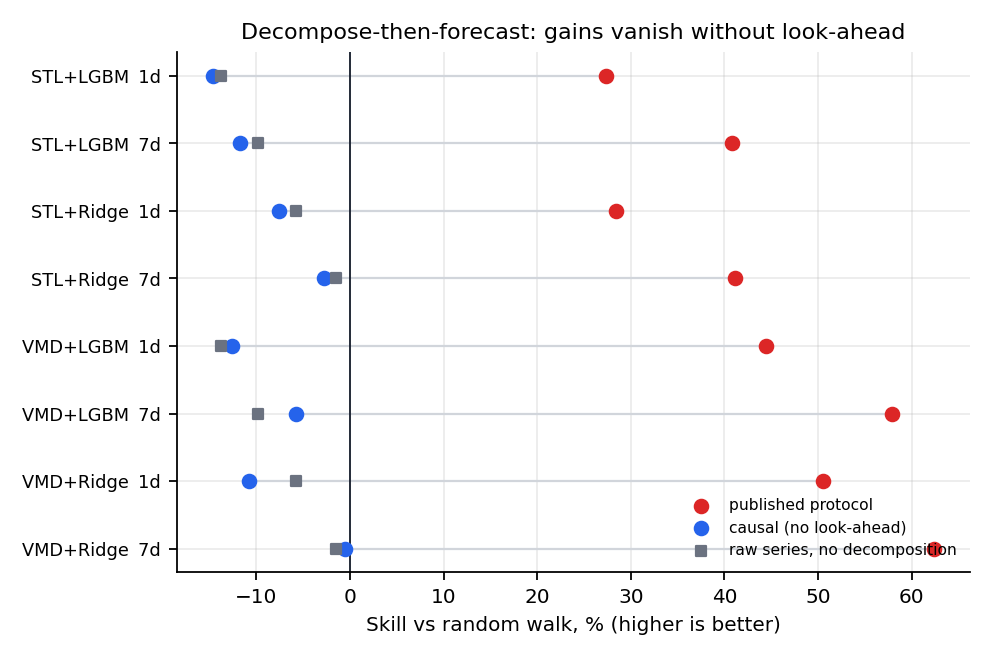
\includegraphics[width=0.85\textwidth,height=7.2cm,keepaspectratio]{figures/fig_leakage.png}
\caption{Skill of decompose-then-forecast models under the published and causal protocols.}
\label{fig:leak}
\end{figure}

\subsection{Sensitivity to assumptions}

Transport cost, spoilage and silent-market discount are assumptions, so ten settings per crop were swept at evaluation time, while models stayed trained under the defaults (Table~\ref{tab:sens}). Across the sweep, models trained on realised outcomes closed 9--36\% of the gap to the oracle relative to the highest price yesterday, while models trained on observed prices stayed between $-8\%$ and $+2\%$. The conclusion in Section~\ref{sec:effects} therefore does not depend on the default economics.

\begin{table}[!t]
\centering
\caption{Range of share of oracle gap closed (relative to the highest price yesterday) across the sensitivity sweep}
\label{tab:sens}
\gentable{tab_sens}
\end{table}

\subsection{Supply shocks}

An event study asked whether large arrival shocks move prices over 3, 7 and 14 days, with placebo circular shifts, minimum detectable effects and Holm correction across \ShockTested{} crop-horizon tests. None was robust (\ShockRobust{}); \ShockSuggestive{} were suggestive (Table~\ref{tab:shock}), and for each the detectable effect was comparable to or larger than the estimate, so power was marginal. These are reported as null results: the data do not support supply-shock trading advice, and the application labels the evidence tier on its shock page.

\begin{table}[!t]
\centering
\caption{Suggestive supply-shock effects, in percent (none survived Holm correction). MDE: minimum detectable effect; placebo $p$ from circular shifts of the shock series}
\label{tab:shock}
\gentable{tab_shock}
\end{table}

\begin{figure}[!t]
\centering
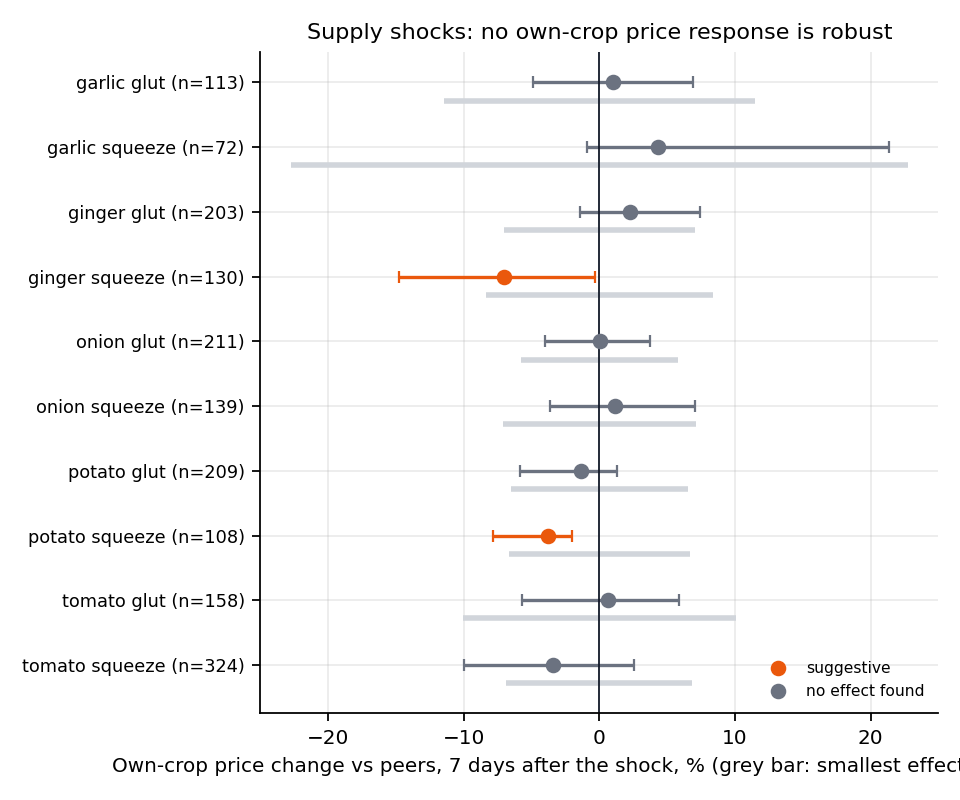
\includegraphics[width=0.85\textwidth,height=7.2cm,keepaspectratio]{figures/fig_shock_effects.png}
\caption{Estimated price effects of arrival shocks with intervals and minimum detectable effects.}
\label{fig:shock}
\end{figure}

\subsection{Cross-commodity spillover}
\label{sec:spill-results}

The engine was run on a weekly panel of five crops over \SpillPeriods{} weeks. Removing the first common factor took out \SpillVar{}\% of the variance of weekly returns, which is the part of co-movement that would otherwise have been read as transmission. Detecting shock episodes from the supply-regime labels then gave \SpillTotalEpisodes{} episodes in every source crop and direction (Table~\ref{tab:spill}), against an evidence floor of eight. All \SpillInsufficient{} of the 40 edges were therefore published as insufficient evidence, no effect size was reported, and the holdout sign-agreement check had no pair to compare (\SpillHoldPairs{} pairs). The engine did what it was built to do, which is to withhold a number it cannot support; the result is that this thesis \emph{does not} show that a shortage in one crop moves another. The AI brief consequently states that spillover evidence is not available rather than citing a link.

\begin{table}[!t]
\centering
\caption{Shock episodes detected per source crop on the weekly panel (floor: 8 episodes)}
\label{tab:spill}
\gentable{tab_spill}
\end{table}

\noindent Zero episodes in all ten source and direction cells is itself a finding about the pipeline, not only about the market: the episode detector depends on supply-regime labels that the preprocessing stage derives from arrivals, and on the real panel no weekly series was labelled squeeze or glut. Whether that reflects a genuinely calm market over 2021--2026, an over-strict labelling threshold, or a labelling stage that is not fed from the real panel has not been resolved, and is listed under future work. The supply-shock event study above, which defines shocks directly from arrivals, did find suggestive same-crop effects, so the data are not shock-free.

\subsection{Decision intelligence and the language layer}
\label{sec:llm-results}

The decision-intelligence service of Section~\ref{sec:intel-method} was tested at two levels. At the code level, 30 unit tests of the brief schema, the evidence bundle, the grounding verifier and the service pass. An invented price is caught; an unknown evidence key is caught; a figure copied from the evidence, or rounded in prose, is accepted; dates and small integers are not treated as claims; a recommended hold is overridden when spoilage outruns the expected gain, in line with the farmer tool's rule; a failing provider falls back to the deterministic one without raising; and withheld spillover evidence is explained in the bundle instead of being shown as zero. At the language level, the writer and judge were evaluated as follows. No study of whether briefs change decisions was done, and the grounding check establishes that figures are traceable to evidence, not that the recommendation is correct; the recommendation itself is the engine's, whose accuracy is reported in Section~\ref{sec:performance-evaluation}.

\LlmExplanations{} explanations (\LlmSentences{} sentences) were generated in English, Kannada and Hindi and judged by an independent model (Table~\ref{tab:llm}). No sentence was rejected by the number validator. The judge rejected 2 of 40 English, 9 of 40 Kannada and 7 of 40 Hindi sentences, which fall back to the original text; the share kept from the model was lower in Kannada and Hindi (0.62--0.88 and 0.68--0.91) than in English (0.83--0.99). To test whether the judge could be trusted, \JudgeBad{} deliberately corrupted explanations and \JudgeGood{} faithful ones were presented: the judge caught \JudgeCaught{} of \JudgeBad{} and wrongly rejected \JudgeFalse{} of \JudgeGood{}. The sample is small, so this shows the judge is not trivially blind rather than that it is reliable. Median latency was \LlmLatency{} seconds per explanation.

\begin{table}[!t]
\centering
\caption{Explanation evaluation by language}
\label{tab:llm}
\gentable{tab_llm}
\end{table}

\subsection{Morning digest}

The digest was tested at two levels. Eight unit tests, using a fake Telegram client with no network, check that every price carries its date and the age of the data, that advice appears only for crops with strong evidence, that the Kannada digest uses Kannada labels, that free-text queries find a crop and a place in the three languages, that onboarding subscribes a farmer and sends the first message, that a farmer who selects no crop is refused, and that unsubscribing removes them from the broadcast. The bot then ran against the real Telegram service: one real account (a team member's) subscribed through the buttons and received two welcome digests, both recorded as sent in the delivery log, and Figure~\ref{fig:digest} shows the message text for tomato and potato at Kolar. A pilot with farmers and a live price feed were not part of this work, so no claim is made about use or effect, and the digest is only as fresh as the last data load (3 days old on 29 October 2026), which it states in its second line.

\begin{figure}[!t]
\centering
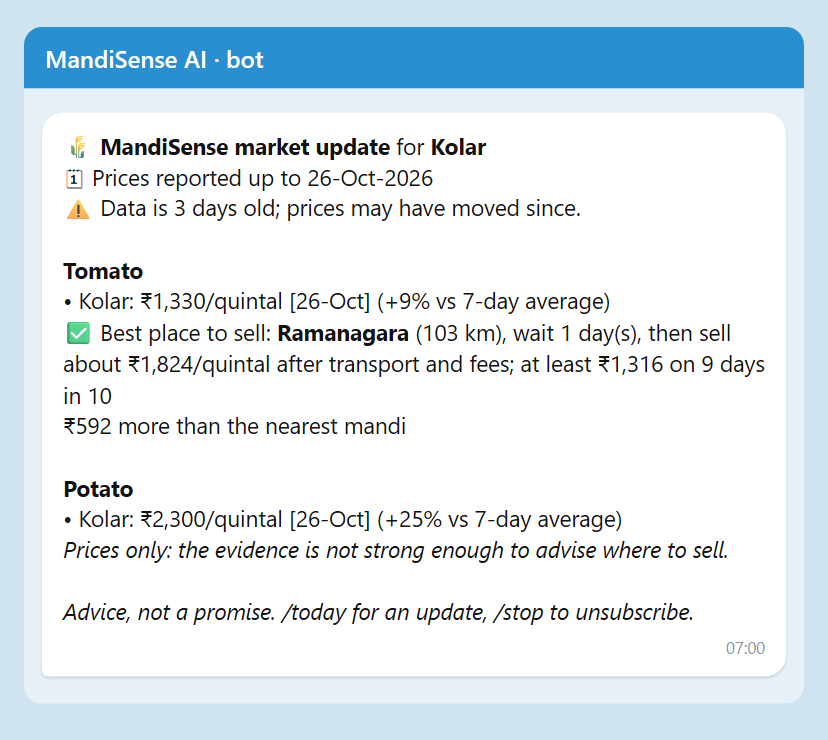
\includegraphics[width=0.34\textwidth]{figures/ins_digest.png}
\caption{The digest message for tomato and potato at Kolar, as sent by the bot (the message text rendered in a chat bubble; the date shown on the first line is the date of the data).}
\label{fig:digest}
\end{figure}

\section{Comparative Analysis}
\label{sec:comparative-analysis}

No published study evaluates mandi choice by regret on real reporting-gap data, so decision results are compared with the heuristics a farmer would plausibly use (Table~\ref{tab:decision}) and with the standard predict-then-optimise baseline, rather than with another paper's numbers. On forecasting, the comparison with published practice is the leakage audit (Table~\ref{tab:leak}) and the foundation-model baseline, and in both the headline accuracy reported for decomposition hybrids was not reproduced under causal evaluation. The contrast between approaches is summarised in Table~\ref{tab:comparative}.

\begin{table}[!t]
\centering
\caption{Comparison of approaches on what they were shown to achieve here}
\label{tab:comparative}
\small
\begin{tabular}{|p{4.3cm}|p{5.2cm}|p{4.9cm}|}
\hline
\textbf{Approach} & \textbf{Result in this study} & \textbf{Qualification} \\ \hline
Nearest mandi, sell today & Lowest revenue in all crops & Common farmer practice \\ \hline
Highest price yesterday & Strong heuristic; 0.17--0.69 of gap closed & Hard to beat in potato \\ \hline
Boosting on observed prices & Indistinguishable from the heuristic & Never sees a silent market \\ \hline
Boosting on realised outcomes & Best or tied-best in all crops & Cost-aware, silence-aware \\ \hline
Neural SPO+ & Tied with boosting & No loss effect found \\ \hline
STL/VMD hybrids, published protocol & +27 to +62\% skill & Disappears causally \\ \hline
Foundation model (zero-shot) & Worse than no change & Daily tomato series \\ \hline
\end{tabular}
\end{table}

\section{Model Optimisation and Innovation}
\label{sec:model-optimization}

\noindent\textbf{What was tried.} Hyper-parameters were tuned with Optuna on a native criterion per method; tuning the most complete model on forecast loss instead of decision regret made no reliable difference. Table~\ref{tab:ablation} lists the four ablations. The reporting head, which models whether a market will report, made decisions \emph{worse} for tomato (Rs~+23 regret, $p=0.012$). Network-silence features, which carry information on whether neighbouring markets are silent, did not reliably help (Rs~$-12$, $p=0.70$). Both were pre-specified hypotheses that failed, and they are reported as such.

\begin{table}[!t]
\centering
\caption{Ablations: change in regret (negative is better) with Holm-adjusted $p$}
\label{tab:ablation}
\gentable{tab_ablation}
\end{table}

\noindent\textbf{What is new.} The contribution that survives testing is the combination: (i) training on realised, silence-aware revenue, which is simple and gave the one robust gain; (ii) floors calibrated online with delayed feedback, which held their nominal level; and (iii) a leak-free evaluation that exposed the inflation in decomposition hybrids. Equation~\ref{eq:aci} is standard adaptive conformal inference~\cite{gibbs2021}; the novelty lies in applying it to selected actions whose outcome resolves $k$ days later.

\noindent\textbf{Limitations of the results.} One region, one source and 5.8 years; revenue parameters are scenarios; ``did not report'' is treated as ``no sale''; and the study is offline, so the effect of farmers acting on the advice is unmeasured.\par
